% \cite{kim2013stereoscopic}
% \cite{bukenberger2018stereo}
% \cite{wysiwyg2002drawing}
% \cite{geiger1995occlusions}
% \cite{cole2008people}
% \cite{rusinkiewicz2008line}
% \cite{hertzmann2000illustrating}
% \cite{raskar1999image}
% \cite{decarlo2003suggestive}
% \cite{raskar2001hardware}
% \cite{yang2010real}
% \cite{decarlo2002stylization}
% \cite{stavrakis2005image}
% \cite{hertzmann1998painterly}
% \cite{northam2012consistent}
% \cite{northam2013stereoscopic}
% \cite{northrup2000artistic}
% \cite{kalnins2003coherent}
% \cite{everitt2001interactive}
% \cite{cole2010two}
% \cite{appel1967notion}
% \cite{DFRS03}
% \cite{INR04}
\chapter{\epsl{}的概念与推导}

\begin{figure}[tbh]
    \centering
    \subfloat[\epslb{}]{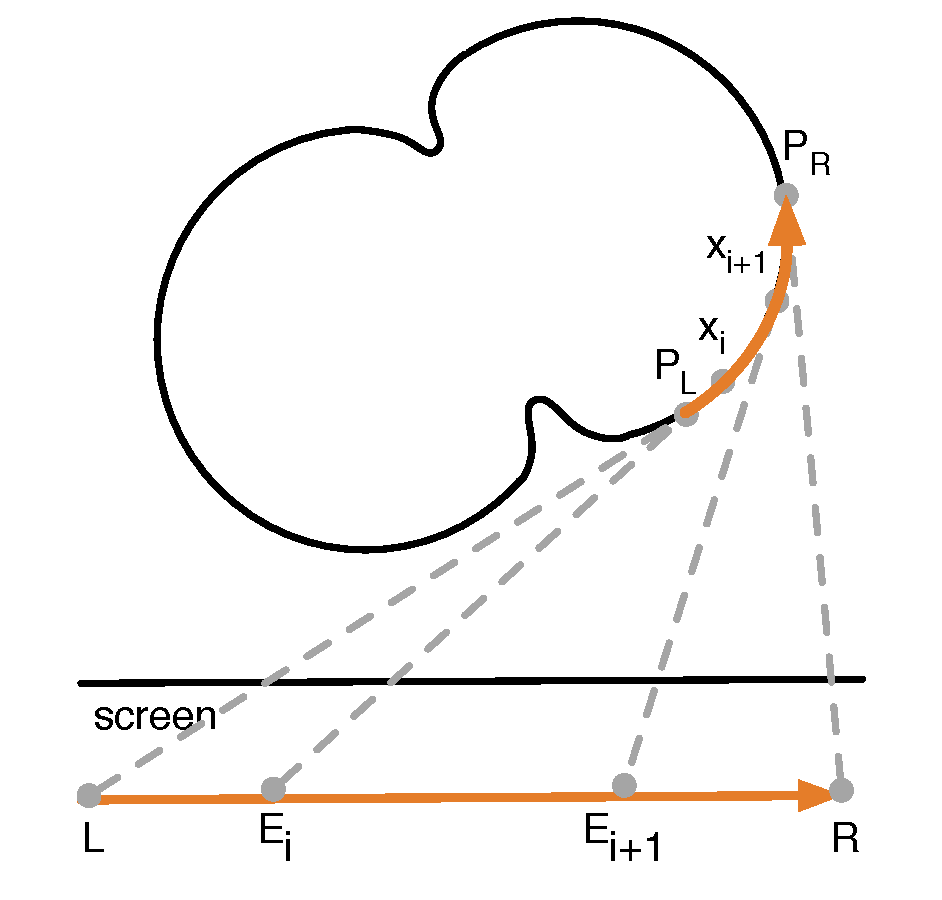
\includegraphics[width=.5\linewidth]{slidable}}
    \hfil
    \subfloat[不是\epslb{}]{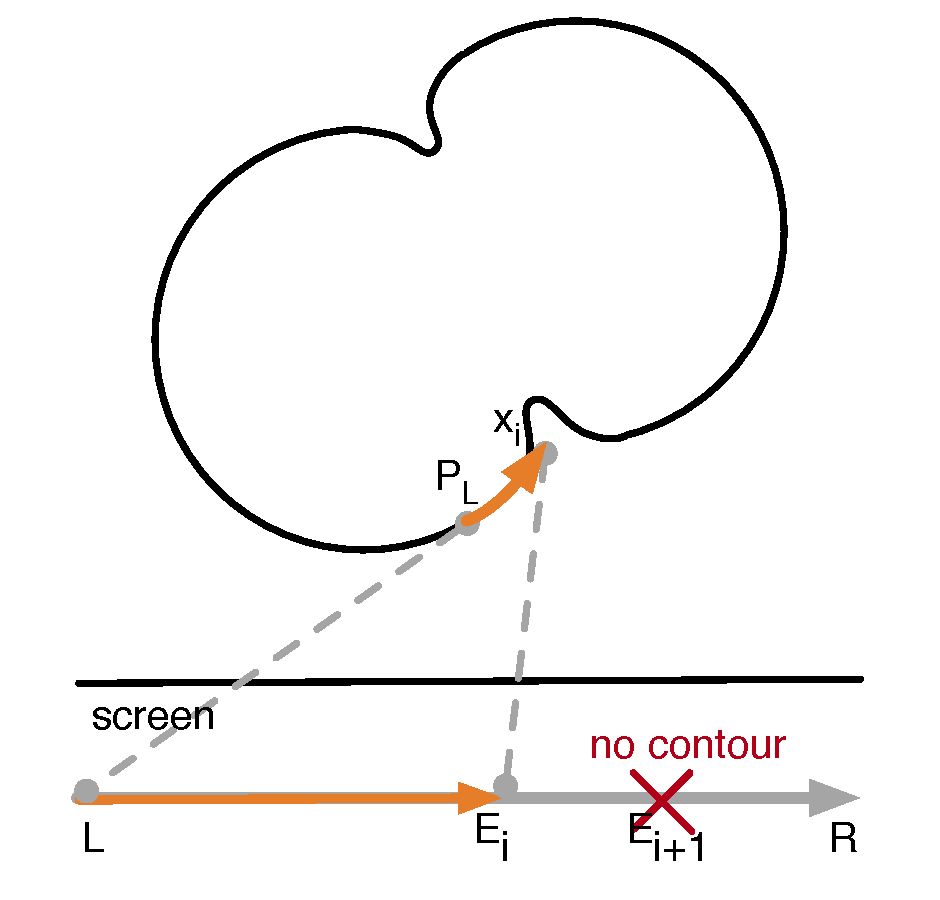
\includegraphics[width=.5\linewidth]{unslidable}}
    \caption{\epsl{}。(a)表示$P_L$是\epslb{},(b)表示$P_L$不是\epslb{}} \label{fig_sim2}
    \label{fig:slidability}
\end{figure}

\begin{figure}[tbh]
    \centering
    \subfloat[\epslb{}]{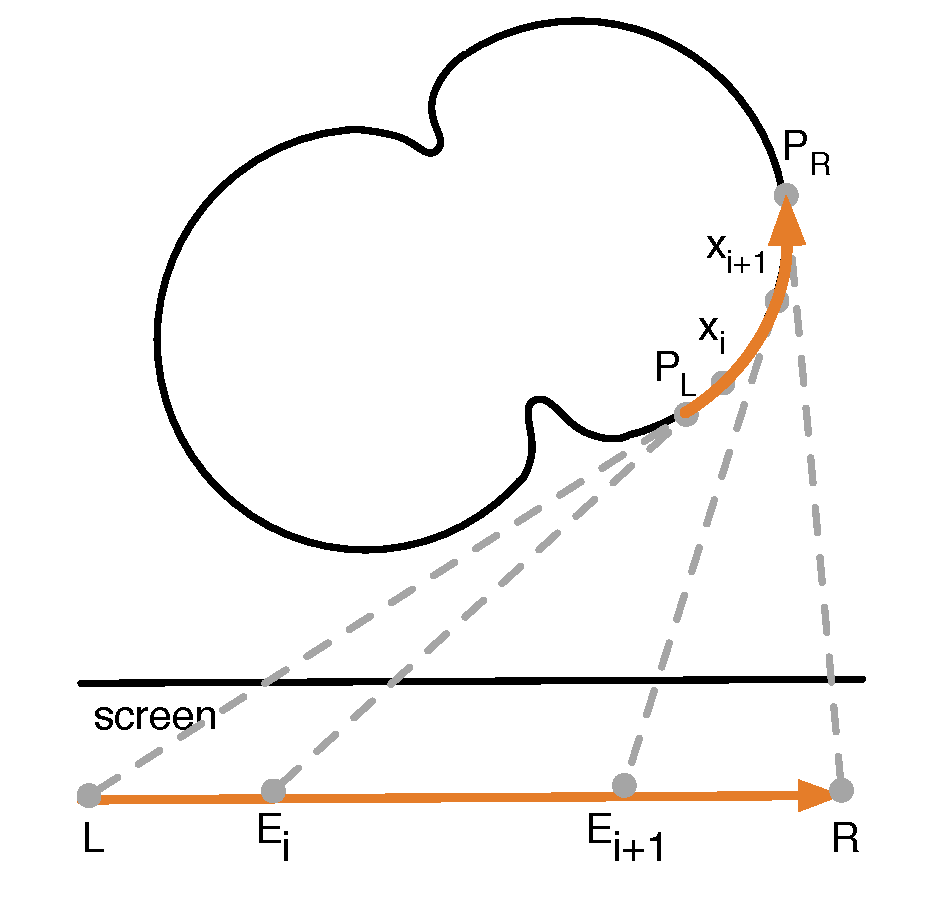
\includegraphics[width=.5\linewidth]{inverse_slidable}\label{fig:inverse_slidable}}
    \hfil
    \subfloat[不是\epslb{}]{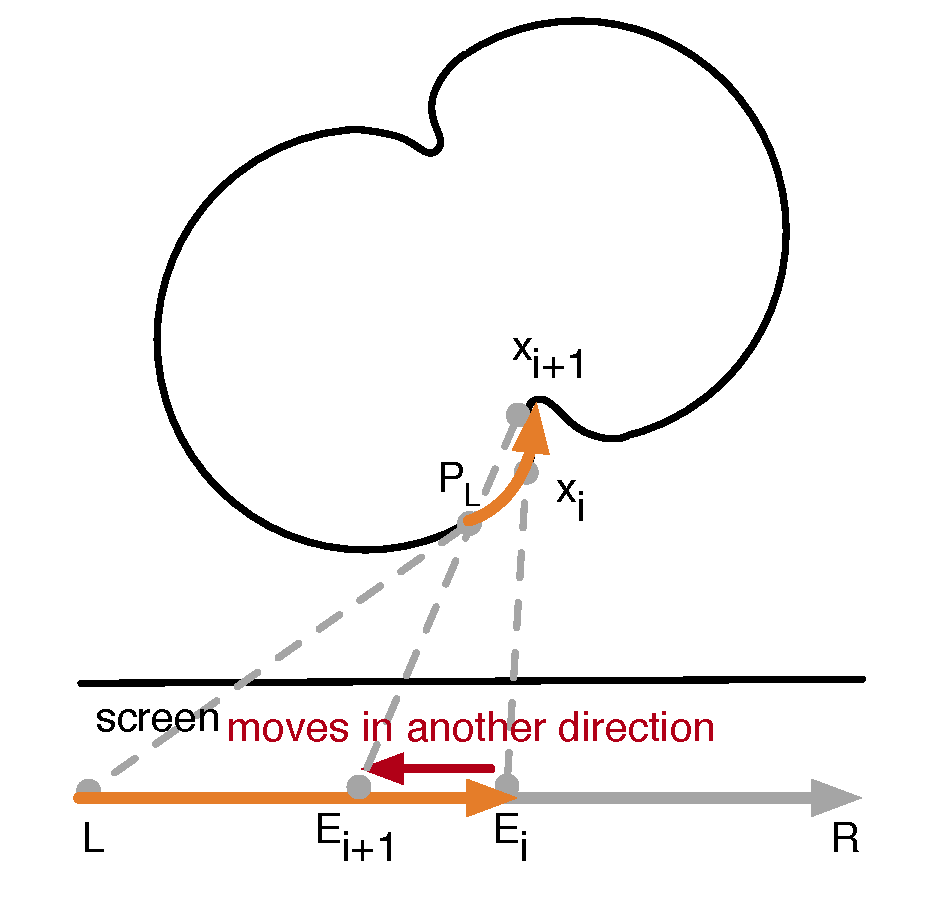
\includegraphics[width=.5\linewidth]{inverse_unslidable}\label{fig:inverse_not_slidable}}
    \caption{\epsl{}的推论。(a)表示$P_L$是\epslb{},(b)表示$P_L$不是\epslb{}} \label{fig:inverse_slidability}
\end{figure}

在这一章节中,本文将先对\citeauthor{kim2013stereoscopic}提出的\epsl{}\cite{kim2013stereoscopic}进行介绍,然后进一步阐述本文在此基础上进行的推导。

\section{\epsl{}}

\epsl{}的定义如下:以\con{}为例,假设$L$和$R$分别表示左眼和右眼,$P_L$和$P_R$分别表示对应的轮廓点(\autoref{fig:slidability})。当视点$E$从$L$向$R$移动,对应的轮廓点也应该从$P_L$向$P_R$移动,它在物体集合表面上移动的曲线称为对极曲线\cite{geiger1995occlusions}。如果对极曲线上的轮廓点能够从$P_L$连续变化到$P_R$,那么$P_L$就是\epslb{}的(\autoref{fig:slidability}(a))。否则,如果对极曲线上的轮廓点能够从$P_L$连续变化到$P_R$,那么$P_L$不是\epslb{}的,不能和对应的轮廓点形成正确的立体视觉(\autoref{fig:slidability}(b)),因此该轮廓点应该在双目绘制的最终结果中被消去。
 
\citeauthor{kim2013stereoscopic}在他们的工作上提出了一种对$P_L$的\epsl{}进行检验的方法。具体来说,他们的方法首先在两眼对应的视点之间插入多个视点并连续地在这些视点上绘制出几何模型的轮廓线。当所有相邻的轮廓点,例如\autoref{fig:slidability}(a)中的$x_i$和$x_{i+1}$,都在一定的区间范围内,那么就$P_L$就是\epslb{}的轮廓点。

需要特别指出的是,以上定义和方法使用\con{}为例进行表述,但是以上定义和方法对于\scon{}也同样成立。在下文的讨论中,如无特别说明,本文也会以\con{}为例进行表述。

\section{\epsl{}的推论}

本文提出的方法拓展了\epsl{}的概念并提出了一个推论:要判定\epsl{},可以通过检查$P_L$到$P_R$的轮廓点的对应视点的轨迹来完成,不需要在$L$和$R$之间采样多个视点进行繁重的计算。

本文提出的方法的出发点如\autoref{fig:inverse_slidability}所示。假设一个轮廓点$x$沿着$P_L$到$P_R$的对极曲线移动,如果$P_L$是\epslb{}的,那么$x$对应的视点会单调地从$L$移动到$R$(\autoref{fig:inverse_slidability}(a))。如果$P_L$不是\epslb{}的,那么对应的视点$E$不会在到达$R$之前保持一直朝着$R$移动(\autoref{fig:inverse_slidability}(b))。

下面分别对\con{}和\scon{}用明确的数学语言给出有关\epsl{}的推论。

\subsection{\con{}}

基于上述的想法,对\epsl{}的判定可以转化为对对应视点的运动轨迹的单调性的检测。具体而言,假设有一个在对极曲线上移动的\conp{}$x$,对应的将其视为\conp{}的视点$E$可以用如下的公式计算:

\begin{equation}\label{eq:viewpoint2}
    {(E - P)}\cdot{N} = 0
\end{equation}

其中$P$和$N$分别表示\conp{}$x$的位置和法线方向。

又因为$E$位于$L$和$R$之间的连线上,所以它的位置可以用一个变量$t$进行以下的参数化:

\begin{equation}\label{eq:viewpoint1}
    E = (1-t)L+t R
\end{equation}

联立\autoref{eq:viewpoint2}和\autoref{eq:viewpoint1}可以得到:

\begin{equation}\label{eq:t1}
t = \frac{(P-L)\cdot{N}}{(R-L)\cdot{N}}
\end{equation}

\autoref{eq:t1}表示$t$是一个关于表面点$x$的函数。当$x$沿着对极曲线运动,$t(x)$就是轮廓点$x$的对应视点的轨迹函数。为了将不同的轨迹函数区分开来,本文使用$t_c(x)$来表示\conp{}的对应视点的轨迹函数,用$t_s(x)$来表示下文将要阐述的\sconp{}的对应的视点的轨迹函数,并用$t(x)$来对以上两种轨迹函数进行合称。

为了进一步讨论轨迹函数$t_c(x)$的单调性,本文将$t_c(x)$的导数形式计算如下:

\begin{equation}\label{eq:derivative}
    % \begin{split}
  t_c' = \frac{(P'\cdot{N}+(P-L)\cdot{N'})((R-L)\cdot{N})}{((R-L)\cdot{N})^2}-\frac{((R-L)\cdot{N'})((P-L)\cdot{N})}{((R-L)\cdot{N})^2}
    % \end{split}
\end{equation}

为了表达上的简洁,本文将\autoref{eq:derivative}中两边的$x$隐去。基于此公式,可以通过$t_c'(x)=0$找到极值点,从而判定轨迹函数的单调性在何时被破坏。该公式还可以作进一步的简化,使得计算起来更加简单。下面从$P(x)$和$N(x)$开始进一步的推导。

\begin{figure}[bth]
    \centering
    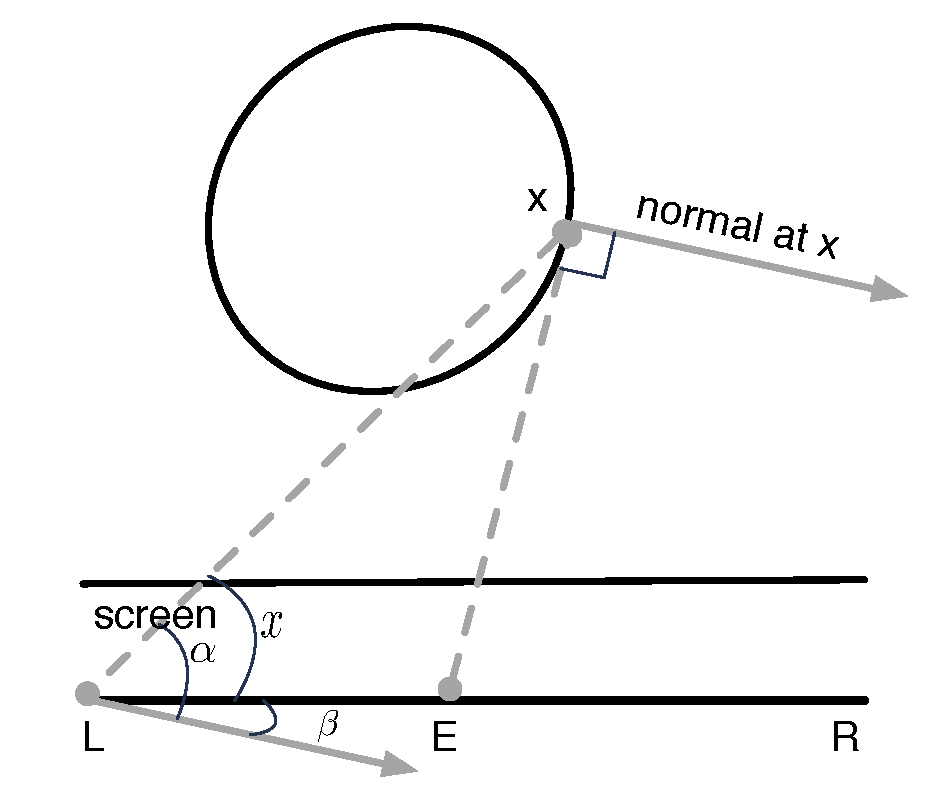
\includegraphics[width=0.6\linewidth]{deduction_t}
    \caption{\label{fig:deduction_t}
    $t$的导数的推导}
\end{figure}  

首先,$x$的位置$P(x)$的导数的方向正是该点的切线方向,换言之,$P'(x)$与法线方向垂直。因此有以下公式:

\begin{equation}\label{eq:perp}
    P'\cdot{N} = 0
\end{equation}

\begin{figure}[bth]
    \centering
    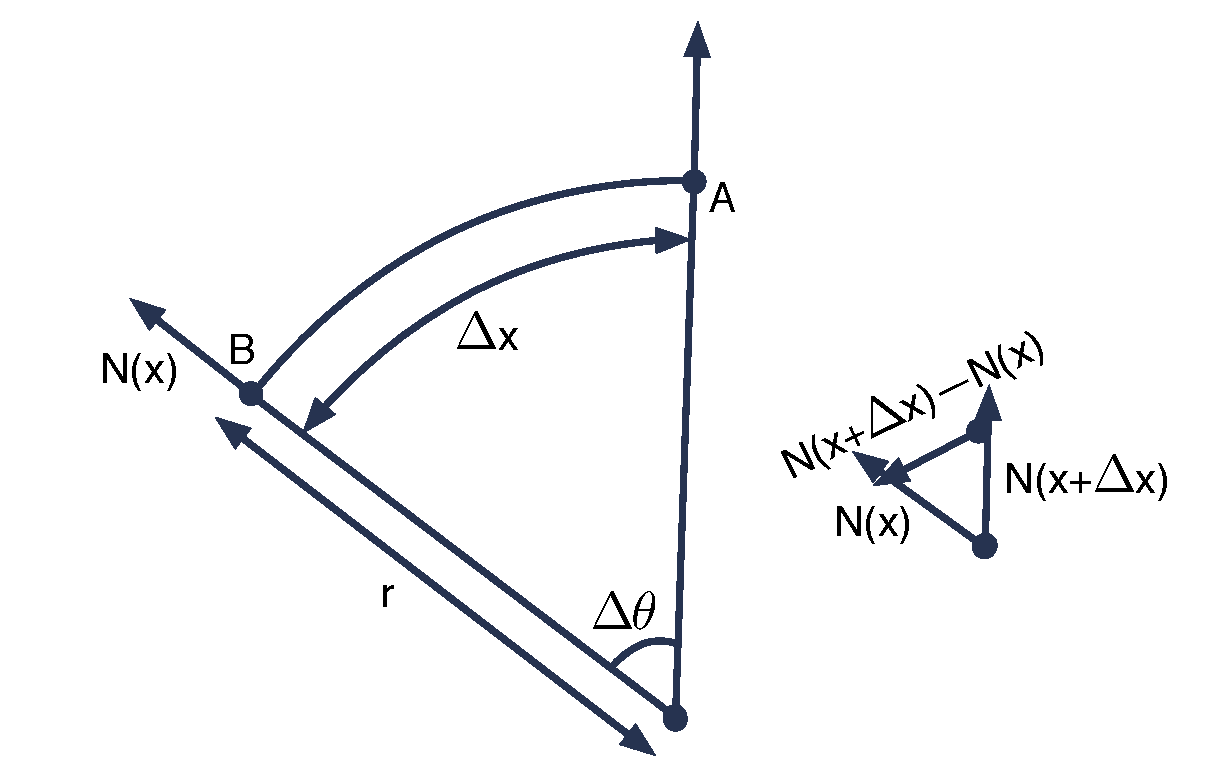
\includegraphics[width=0.6\linewidth]{deduction_n}
    \caption{\label{fig:deduction_n}
    曲线的法线导数的推导}
\end{figure}

再者,$x$的法线方向$N(x)$的导数可以进行以下的推导得出。首先,$N(x)$可以作为单位法线使用,原因如下:

\begin{equation}
    t_c = \frac{(P-L)\cdot{N}}{(R-L)\cdot{N}} = \frac{(P-L)\cdot{\frac{N}{|N|}}}{(R-L)\cdot{\frac{N}{|N|}}}
\end{equation}

接着,正如\autoref{fig:deduction_n}所示,当$P(x+\Delta x)$从$A$移动到$B$,$N(x)$,$N(x+\Delta x)$和$N(x+\Delta x)$ - $N(x)$组成来一个等腰三角形,因为$N(x)$和$N(x+\Delta x)$都是单位法线。因此可以得出:

\begin{equation}
    |N(x+\Delta x) - N(x)| = \Delta\theta \cdot 1 = \Delta\theta = |N'(x)\Delta x|
\end{equation}

又由于$\Delta x \to 0$,所以

\begin{equation}\label{eq:curvature}
    |N'(x)| = \lim_{x \to 0}\frac{\Delta\theta}{\Delta x} = \lim_{x \to 0}\frac{\Delta\theta}{r\Delta\theta} = \frac{1}{r} = C(x)
\end{equation}

其中$C(x)$表示对极曲线上一点$x$的曲率。另外,当$\Delta x \to 0$,$|N(x+\Delta x) - N(x)|$的方向趋近于与法线$N(x)$的方向垂直,因此可以得到$N'(x) \perp N(x)$。假设 $\alpha$表示$P(x)-L$和$N(x)$之间的夹角,$\beta$表示$R-L$和$N(x)$之间的夹角,可以进行如下的转化:

\begin{equation}\label{eq:alpha}
(P-L)\cdot{N'} = |P-L|{|N'|}\cos{(\alpha+\frac{\Pi}{2})} = |P-L|{|N'|}\sin\alpha
\end{equation}

\begin{equation}\label{eq:beta}
(R-L)\cdot{N'} = |R-L|{|N'|}\cos{(\beta+\frac{\Pi}{2})} = |R-L|{|N'|}\sin\beta
\end{equation}

结合\autoref{eq:derivative},\autoref{eq:perp},\autoref{eq:curvature},\autoref{eq:alpha}和\ref{eq:beta},可以得到:

\begin{equation}\label{eq:final}
\begin{split}
t_c' & = \frac{C|P-L||N|\sin\alpha|R-L||N|\cos\beta-C|R-L||N|\sin\beta|P-L||N|\cos\alpha}{((R-L)\cdot{N})^2} \\
& = \frac{C|P-L||R-L||N|^2(\sin\alpha\cos\beta-\sin\beta\cos\alpha)}{((R-L)\cdot{N})^2} \\
& = \frac{C|P-L||R-L||N|^2\sin(\alpha-\beta)}{((R-L)\cdot{N})^2} \\
& = \frac{C|P-L||R-L||N|^2\sin(\gamma)}{((R-L)\cdot{N})^2}
\end{split}
\end{equation}

正如\autoref{fig:deduction_t}所示,$\gamma$是$P(x)-L$和$R-L$之间的夹角。由于$x$ 位于$L$与$R$连线的正前方,$sin\gamma$的值恒大于0。因此,$t_c'(x)$的符号只与$C(x)$有关。

需要明确指出的是,由于三维模型的不连续性,$t_c'(x)=0$在模型上出现的位置并不是连续的。因此,本文将通过$t_c'(x-)t_c'(x+) < 0$而不是$t_c'(x)=0$来找出极值点。

在本文设计的方法中,会将对极曲线上的\conp{}投影到左眼和右眼对应的图像,再沿着对极线(epipolar line)而不是物体空间中的对极曲线(epipolar curve)进行搜索。这样一来,即可计算出极值点并存储到图像空间,从而在图像空间实现\epsl{}的判定。

\subsection{\scon{}}
\label{sec:suggestive_contour_math}
通过检测对应视点的轨迹的想法同样可以应用到\scon{}上。\scon{}的定义如下:

\begin{align}
  \kappa_r &= 0 \label{eq:Kr} \\
  D_w\kappa_r &> 0 \label{eq:DwKr} 
\end{align}

其中$\kappa_r$表示表面上一点的径向曲率,$D_w\kappa_r$表示$\kappa_r$的方向导数。更确切地说,$\kappa_r$是视线方向$V$在切平面上的投影$W$的方向上的法向曲率。法向曲率以及方向导数的概念已经在\autoref{sec:diff_geo}中进行说明,在此不再赘述。$\kappa_r$可以用以下形式表示为关于主曲率(principal curvature)和$W$的函数:

\begin{equation}\label{eq:normal curvature}
    \kappa_r = \kappa_1cos^2\phi+\kappa_2sin^2\phi
\end{equation}

其中$\kappa_1$和$\kappa_2$是两个主曲率,$\phi$是$W$的方向与$\kappa_1$对应的主曲率方向(principal curvature direction)。假设$\kappa_1$和$\kappa_2$满足$\kappa_1\kappa_2 \leq 0$,可以按照以下形式计算出满足$\kappa_r = 0$的$W$:

\begin{equation}\label{eq:w}
    W = \pm\sqrt{\frac{\kappa_2}{\kappa_2-\kappa_1}}D_1\pm\sqrt{\frac{-\kappa_1}{\kappa_2-\kappa_1}}D_2
\end{equation}

其中$D_1$和$D_2$是分别是对应的主曲率的方向。尽管\autoref{eq:w}中$\kappa_r = 0$的解有四个,但是只有其中两个可以是$L$和$R$之间一个视点$E$的视线方向的投影。对于每个$W$,将某个表面点视为\sconp{}的视点$E$必须满足:

\begin{equation}\label{eq:suggestive viewpoint}
    {(E - P)}\cdot{M} = 0
\end{equation}

其中$M$是$W$和表面法线$N$的叉积。不难看出,由于\autoref{eq:suggestive viewpoint}的形式和\autoref{eq:t1}一致,同样地,可以将视点$E$用一个参数$t$参数化成\autoref{eq:viewpoint1}的形式并推导出$t$的表达式:

\begin{equation}\label{eq:suggestive trajectory}
    t = \frac{(P-L)\cdot{M}}{(R-L)\cdot{M}}
\end{equation}

该公式表示了\scon{}的对应视点的轨迹函数,也就是$t_s(x)$。同样地,基于$t_s(x)$可以计算出极值点从而对\scon{}的\epsl{}进行判定。然而,与\con{}不同的是,对于每个\sconp{}会有两个对应的视点将其视为\sconp{},所以$t_s(x)$是一个多值函数(multivalued function)。关于\scon{}的极值点的计算细节将在\ref{sec:suggestive_contour_algorithm}中进一步阐述。

另外,关于$t_s(x)$的推导是建立在$\kappa_1\kappa_2 \leq 0$的假设的前提下的,另一个条件$D_w\kappa_r>0$还没有考虑在内。再者,在实际实现中,还会用以下的条件来进一步限制\scon{}的出现范围:

\begin{equation}\label{eq:cosNdotV}
  cos^{-1}(N\cdot{V}) > \theta_c 
\end{equation}

对于那些不符合三个条件的表面点,不存在对应的视点将其视为\sconp{}。换言之,$t_s(x)$的区间端点有三种:

\begin{enumerate}
\item $\kappa_1\kappa_2 = 0$
\item $D_w\kappa_r = 0$
\item $cos^{-1}(N\cdot{V}) = \theta_c$
\end{enumerate}

除了极值点以外,这些区间端点也会破坏对应视点的轨迹的单调性。因此,对于\scon{}来说,要实现\epsl{}的判定,除了计算出极值点外,还需要计算出这些区间端点来作进一步的判断。